\documentclass[11pt]{article}
\usepackage[margin=1in]{geometry}
\usepackage{amsmath,amssymb,amsthm}
\usepackage{hyperref}
\usepackage{tikz}
\ifdefined\pdftrailerid\pdftrailerid{}\fi

\newtheorem{theorem}{Theorem}
\newtheorem{proposition}{Proposition}
\newtheorem{lemma}{Lemma}
\newtheorem{corollary}{Corollary}
\theoremstyle{remark}
\newtheorem{remark}{Remark}
\theoremstyle{plain}
\newtheorem{question}{Question}

\newcommand{\R}{\mathbb{R}}
\newcommand{\Kcal}{\mathcal{K}}
\newcommand{\Lcal}{\mathcal{L}}
\newcommand{\Pcal}{\mathcal{P}}
\DeclareMathOperator{\Gr}{Gr}
\DeclareMathOperator{\St}{St}

\title{Discriminant Varieties for Stick Knots and Links}
\author{Alexander Kolpakov \and Igor Rivin}
\date{23 October 2026}

\begin{document}

\maketitle

\begin{abstract}
How many knot types can be built from a fixed budget of straight sticks?  We
give, to our knowledge, the first explicit determination of their asymptotic
growth order.  Writing \(\Kcal_N\) for the knot types realizable with at most
\(N\) sticks, we prove
\[
 N^{(2/3+o(1))N}\le |\Kcal_N|\le N^{3N+o(N)}.
\]
Thus \(\log|\Kcal_N|=\Theta(N\log N)\).  Our direct discriminant
argument turns polygonal
self-intersection into a sparse real-algebraic chamber problem in only
linearly many dimensions.  A Garside refinement of the Malyutin--Stupakov
pure-braid injection gives the \(2/3\) lower exponent, already among prime
satellite knots.  The result
ties knot topology directly to real algebraic geometry, fewnomial structure,
and permutation combinatorics.
\end{abstract}

\section{Introduction}

Let \(p_1,\ldots,p_N\in\R^3\) be labeled vertices joined cyclically by straight
segments.  The space of embedded \(N\)-gons is the complement of a
self-intersection discriminant.  Its connected components are sometimes called
geometric knot types: two polygons in the same component are connected by an
isotopy through \(N\)-gons.  Calvo computed this space for \(N=6,7\), showing in
particular that geometric equivalence is finer than ordinary topological knot
type \cite{Calvo}.  The exact number of components is unknown in general.

The semialgebraic starting point is also already present in Calvo's work:
for every pair of non--incident edges, the possible-intersection locus is
described there as a codimension-one cubic semialgebraic piece, with additional
inequalities selecting intersections of the segments rather than merely their
supporting lines.  Thus neither the polygon-space discriminant nor its
semialgebraicity is claimed as new here.  Our upper bound is a quantitative
extraction from that model: we retain the binomial dependence on the number of
walls in a refined sign-condition component estimate.

The purpose of this note is to isolate what can be proved by elementary
semialgebraic methods.  The basic facts are:
\begin{itemize}
    \item the discriminant is semialgebraic and has explicit low-degree chart
    equations;
    \item knot type is constant on each chamber of the complement;
    \item every knot type with stick number at most \(N\) occurs in at least one
    chamber of positive measure; and
    \item determinant-related sign-condition bounds, with their binomial
    factor retained, give
    \[
        |\Kcal_N|\le (A N)^{3N}=N^{3N+o(N)};
    \]
    \item combined with the factorial arc-index lower bound of
    Malyutin--Stupakov, the chamber estimate makes explicit the logarithmic growth
    order
    \(\log|\Kcal_N|=\Theta(N\log N)\), equivalently the scale
    \(N^{\Theta(N)}\);
    \item a further extraction from the Malyutin--Stupakov pure-braid
    construction, using Garside normal forms and an explicit factorial-size
    family of doubly alternating permutations, sharpens the lower side to
    \(|\Kcal_N|\ge N^{(2/3+o(1))N}\), already among prime satellite knots;
    and
    \item after summing over component decompositions, there are at most
    \(N^{4N+o(N)}\) ordinary links with at most \(N\) total sticks.
\end{itemize}
The determinant form of the crossing walls is the reason that one expects a
substantially structured chamber-count problem rather than an arbitrary
arrangement of high-degree hypersurfaces.

A generic projection of an \(N\)-stick polygon has at most \(N(N-3)/2\)
crossings, and classical exponential enumeration by crossing number gives the
baseline \(|\Kcal_N|\le\exp(O(N^2))\) \cite{FreedmanHeWang}.  More recently,
Gros--Ramirez Alfonsin proved that the strong geometry of a generic vertex
configuration determines its polygonal-knot type \cite{GrosRamirez}.  In
principle, their reconstruction theorem could be combined with sign-pattern
estimates to obtain counting bounds.  Our proof takes a different route,
counting chambers of the self-intersection discriminant directly, and is
independent of that reconstruction theorem.

Our contribution is the much sharper direct stick-space estimate obtained by
making Calvo's semialgebraic discriminant model quantitative:
\[
 |\Kcal_N|\le N^{(3+o(1))N}.
\]
Together with the lower construction, this gives, to our knowledge, the first
explicit theorem establishing the sharp logarithmic growth order
\(\log|\Kcal_N|=\Theta(N\log N)\).  The Garside construction below gives
the explicit lower exponent \(2/3\).  We use established geometric and
sign-condition inputs to obtain the counting theorem; the discriminant model
and the general real-algebraic component theorem retain their original
attributions.
Randell--Simon--Tokle directly studied the counting
function by polygon length and proved an exponential lower bound, but no
comparable factorial lower bound \cite{RandellSimonTokle}.  Millett later
listed the corresponding question for equilateral polygons as an open problem
and reported that no useful estimate by edge number was then available
\cite[Problem 5.2]{MillettPhysical}.  Recent computational work concerns upper
bounds for individual stick numbers rather than this counting function
\cite{CantarellaEtAl2025}.
\section{Normalized stick-knot parameter space}

Let
\[
    H=\mathbf{1}^{\perp}\subset\R^N.
\]
After subtracting the centroid of the vertices, the three coordinate rows of a
full-dimensional polygon lie in \(H\).  Applying an invertible linear change of
coordinates in \(\R^3\), one may normalize the row Gram matrix to the identity.
This leads to the Stiefel model
\[
    X_N=\St_3(H)
    =
    \{Q\in\R^{3\times N}: Q\mathbf{1}=0,\; QQ^T=I_3\}.
\]
The columns \(q_i=Qe_i\in\R^3\) are the normalized vertices.  Since
\(\dim H=N-1\),
\[
    \dim X_N
    =
    3(N-1)-\frac{3\cdot4}{2}
    =
    3N-9.
\]
Quotienting by \(SO(3)\) gives the oriented Grassmannian
\[
    \widetilde{\Gr}_3(H)=X_N/SO(3),
    \qquad
    \dim \widetilde{\Gr}_3(H)=3N-12.
\]
This does not change chamber counts: the quotient is a locally trivial bundle
with connected fiber \(SO(3)\), and rotations move a polygon inside the same
embedding chamber.  This normalization is geometrically natural, although the
upper bound below is proved directly in the unsliced vertex space.
Quotienting by all of \(O(3)\), on the other hand, identifies mirror images.

\section{Local equations for crossing walls}

Consider two non--incident directed edges \(ab\) and \(cd\), and write
\[
    v=p_b-p_a,\qquad w=p_d-p_c,\qquad r=p_c-p_a.
\]
In the \(xy\)-projection chart, set
\[
    D=\det\begin{pmatrix}
        x_b-x_a & x_d-x_c\\
        y_b-y_a & y_d-y_c
    \end{pmatrix},
\]
\[
    N_\lambda=\det\begin{pmatrix}
        x_c-x_a & x_d-x_c\\
        y_c-y_a & y_d-y_c
    \end{pmatrix},\qquad
    N_\mu=\det\begin{pmatrix}
        x_c-x_a & x_b-x_a\\
        y_c-y_a & y_b-y_a
    \end{pmatrix}.
\]
When \(D\ne0\), the two projected supporting lines meet at parameters
\[
    \lambda=\frac{N_\lambda}{D},\qquad
    \mu=\frac{N_\mu}{D}.
\]
The projected crossing lies in the interiors of both segments precisely when
\[
    N_\lambda(D-N_\lambda)>0,\qquad
    N_\mu(D-N_\mu)>0.
\]
The height difference at the crossing is
\[
    h=z_a+\lambda(z_b-z_a)-z_c-\mu(z_d-z_c).
\]
Clearing denominators gives
\[
    F_{ab,cd}
    =
    D(z_a-z_c)
    +N_\lambda(z_b-z_a)
    -N_\mu(z_d-z_c).
\]
Equivalently, up to sign,
\[
    F_{ab,cd}
    =
    \det(p_b-p_a,\;p_d-p_c,\;p_c-p_a).
\]
This is the affine orientation determinant of the four vertices
\(p_a,p_b,p_c,p_d\), up to sign.  Thus each over/under wall is not merely a
low-degree equation: it is one of the determinant walls governing the order
type of the vertex configuration.  As a polynomial in the coordinate variables,
it has at most \(24\) monomial terms before cancellation.  The same construction
is used in the \(xz\)- and \(yz\)-projection charts.  The cases where the
relevant \(2\times2\) projected determinant vanishes are lower-dimensional
chart degeneracies.  They may be included in a full chartwise sign
description, but are not needed for the enlarged coordinate-free wall family
used in Theorem~\ref{thm:upper}.

\section{The discriminant and its chambers}

Let \(\Delta_N\subset X_N\) be the set for which the cyclic piecewise-linear
map is not an embedding.  Thus an edge may collapse, adjacent edges may meet
away from their common endpoint, or two combinatorially non--incident edges may
meet.  The last condition says that, for some such pair \(ab,cd\), there are
\(\lambda,\mu\in[0,1]\) with
\[
    p_a+\lambda(p_b-p_a)=p_c+\mu(p_d-p_c).
\]
Edge collapse and adjacent-edge overlap have similarly elementary polynomial
descriptions.  These first-order formulas use only polynomial equalities and
inequalities with existentially quantified segment parameters, so the
Tarski--Seidenberg theorem \cite[Section 2.2]{BochnakCosteRoy} implies that
\(\Delta_N\) is semialgebraic.  This formulation includes the adjacent
backtracking degeneracy that is missed if one mentions only non--incident edge
pairs.

Define
\[
    C_N=b_0(X_N\setminus\Delta_N),
\]
the number of embedding chambers.  For a knot type \(K\), let \(C_N(K)\) be
the number of chambers in which the polygon has type \(K\).

\begin{proposition}[Chambers carry one knot type]\label{prop:chambers}
The ambient isotopy class of the cyclic polygon is constant on each connected
component of \(X_N\setminus\Delta_N\).
\end{proposition}

\begin{proof}
Connected semialgebraic sets are semialgebraically path-connected, so two
points of a chamber can be joined by a path in
\(X_N\setminus\Delta_N\).  Such a path is a one-parameter family of embedded
polygonal curves with fixed cyclic combinatorics.  For a sufficiently fine
subdivision of the parameter interval, consecutive polygons are close enough
that the straight-line interpolation of corresponding vertices remains
embedded.  This gives an isotopy through embedded polygonal curves, and the
ambient isotopy extension theorem \cite{EdwardsKirby} gives ambient isotopy of
the endpoints.
\end{proof}

\begin{remark}[Generic walls]
At a smooth codimension-one point of a single wall \(F_{ab,cd}=0\), with
\(D\ne0\), \(0<\lambda,\mu<1\), and no simultaneous degeneracy, crossing the
wall changes the sign of the height difference \(h=F_{ab,cd}/D\).  Thus the
two adjacent diagrams differ by one over/under switch.  This is a local
statement; it does not imply that all crossing assignments in a large diagram
are independently realizable.
\end{remark}

\section{Support of the knot type map}

Let \(\operatorname{stick}(K)\) denote the stick number of a knot type \(K\).
This is the minimum number of straight segments needed in a polygonal
representative of \(K\); see, for example, the standard tables and references in
KnotInfo \cite{KnotInfoStick} and the stick-number work of Adams et al.
\cite{AdamsStick}.

\begin{theorem}[Support theorem]\label{thm:support}
For \(N\ge4\), the image of the knot type map
\[
    \tau_N:X_N\setminus\Delta_N\longrightarrow
    \{\text{ambient isotopy classes of knots}\}
\]
is exactly
\[
    \Kcal_N=\{K:\operatorname{stick}(K)\le N\}.
\]
Moreover, if \(K\in\Kcal_N\), then \(\tau_N^{-1}(K)\) contains a nonempty open
subset of \(X_N\).  In particular it has positive measure for the natural
\(O(N-1)\)-invariant Riemannian volume on \(X_N\), and
\[
    C_N(K)\ge1
    \quad\Longleftrightarrow\quad
    \operatorname{stick}(K)\le N.
\]
\end{theorem}

\begin{proof}
If \(Q\in X_N\setminus\Delta_N\), then its columns form an embedded polygon
with \(N\) sticks.  Hence the represented knot type \(K=\tau_N(Q)\) satisfies
\(\operatorname{stick}(K)\le N\).

Conversely, suppose \(\operatorname{stick}(K)\le N\).  Choose a polygonal
representative of \(K\) with at most \(N\) sticks and subdivide edges, if
necessary, to obtain exactly \(N\) labeled vertices.  After an arbitrarily small
ambient isotopy, assume that the centered coordinate rows span a
three-dimensional subspace of \(H\).  Let \(M\in\R^{3\times N}\) be the matrix
of centered vertex coordinates.  Then \(M\mathbf 1=0\) and \(MM^T\) is positive
definite.  Put
\[
    A=(MM^T)^{1/2},\qquad Q=A^{-1}M.
\]
Then \(Q\mathbf 1=0\) and \(QQ^T=I_3\), so \(Q\in X_N\).  The original centered
polygon is the image of the \(Q\)-polygon under the orientation-preserving
linear map \(A\).  Therefore \(Q\) represents the same knot type \(K\), and
\(Q\notin\Delta_N\).

Finally, stability of PL embeddings under sufficiently small vertex
perturbations \cite{EdwardsKirby} gives a neighborhood of \(Q\) in \(X_N\)
representing the same knot type.  Concretely, non--incident edges have
positive separation, every edge is nonzero, and local injectivity at the
finitely many adjacent pairs persists; at a straight subdivision vertex the
two outgoing directions have strictly negative dot product.  Nonempty open
subsets of the compact smooth manifold \(X_N\) have positive natural
\(O(N-1)\)-invariant Riemannian volume.
\end{proof}

\section{A determinantal semialgebraic upper bound}

\begin{theorem}[Stick-knot upper bound]\label{thm:upper}
There exists an absolute constant \(A>0\) such that, for every integer
\(N\ge4\),
\[
    |\Kcal_N|\le (A N)^{3N}.
\]
Consequently \(|\Kcal_N|\le N^{3N+o(N)}\) as \(N\to\infty\).
\end{theorem}

\begin{proof}
Write \(e_i=p_{i+1}-p_i\), with indices read cyclically.  There are
\[
    r_N=\frac{N(N-3)}{2}
\]
unordered pairs of non--incident edges.  For each such pair put
\[
    f_{ij}=\det(e_i,e_j,p_j-p_i),
\]
and, for each adjacent pair, put
\[
    h_i=\|e_i\times e_{i+1}\|^2.
\]
The \(f_{ij}\) have degree three and the \(h_i\) have degree four.  If none
vanishes, consecutive edges are nonzero and noncollinear, hence meet only at
their prescribed common endpoint.  Two non--incident segments cannot meet
either: an intersection would make their two directions and displacement
coplanar and force the corresponding \(f_{ij}\) to vanish.  Thus the complement
of these
\[
    s=r_N+N=\frac{N(N-1)}2
\]
algebraic walls consists entirely of embedded polygons.  It is harmless that
these enlarged walls also delete benign coplanar configurations and straight
subdivisions.

Let \(G_N\subset(\R^3)^N\cong\R^{3N}\) be the complement of this enlarged
wall family.  Every knot in \(\Kcal_N\) has a representative in \(G_N\):
subdivide to exactly \(N\) vertices and make an arbitrarily small generic
perturbation.  PL stability preserves knot type, while a generic perturbation
avoids the finitely many nonzero wall polynomials.  On the other hand, every
point of \(G_N\) is an embedded polygon by the preceding paragraph.

The knot-type map on \(G_N\) is constant on path components.  Indeed, a path
in \(G_N\) is a one-parameter family of embedded polygonal curves, and ambient
isotopy extension identifies its endpoints.  Since \(G_N\) is open in a
Euclidean space, connected components and path components agree.  The induced
map
\[
    \pi_0(G_N)\longrightarrow\Kcal_N
\]
is therefore surjective, and
\[
    |\Kcal_N|\le b_0(G_N).
\]

On \(G_N\) the sign of every wall is locally constant, so \(b_0(G_N)\) is the
sum of the component counts of its realizable strict sign conditions.
Dimension-sensitive cell bounds retaining the
essential \((s/m)^m\) dependence go back to Pollack--Roy
\cite{PollackRoy}.  We use the part of the sign-condition theorem that is lost in the cruder
\(s^m\) notation.  The explicit Barone--Basu bound
\cite[Theorem 1.1]{BaroneBasu}, specialized to \(s\) polynomials of degree at
most four on \(\R^m\), implies, after absorbing fixed-degree factors into
an absolute constant \(B\),
\[
 b_0(G_N)
 \le B^m\sum_{j=0}^{m}4^j\binom{s+1}{j}.
\]
Explicitly, take
\(\mathcal Q=\varnothing\), \(V=\R^m\), \(k'=k=m\), and \(d=4\) in their
formula (with any fixed vacuous \(d_0\), say \(2\)).  Its \(j\)-th auxiliary
factor is bounded using
\(\binom{m+1}{j+1}\le2^{m+1}\), with all remaining fixed-degree factors
absorbed into \(B^m\).

For exact agreement with the Lean development, index a redundant family of
\[
    S=N+N^2
\]
slots: use the \(N\) adjacent walls above, put the appropriate determinant in
each relevant ordered-pair slot, and put the constant polynomial \(1\) in
every irrelevant slot.  This leaves the nonzero locus unchanged.  With
\(m=3N\), one has \(m\le(S+1)/2\) for \(N\ge5\), and hence
\[
 \sum_{j=0}^{m}4^j\binom{S+1}{j}
 \le (m+1)4^m\binom{S+1}{m}
 \le (m+1)\left(\frac{4e(S+1)}m\right)^m.
\]
Since \((S+1)/m=O(N)\), enlarging the absolute constant absorbs the factor
\(m+1\) and gives \(b_0(G_N)\le(AN)^{3N}\).  Enlarging \(A\) also covers
\(N=4\).  This proves the first estimate.

\end{proof}

\begin{corollary}[Comparison with geometric chambers]\label{cor:knot-types}
For the normalized polygon space of the preceding sections,
\[
    |\Kcal_N|
    \le
    \sum_{K\in\Kcal_N} C_N(K)
    =
    C_N.
\]
\end{corollary}

\begin{proof}
By Theorem~\ref{thm:support}, every \(K\in\Kcal_N\) is represented by at least
one chamber.  By Proposition~\ref{prop:chambers}, each chamber represents only
one topological knot type.  Therefore the chamber count bounds the number of
represented knot types from above.
\end{proof}

\begin{theorem}[Asymptotic growth order]\label{thm:asymptotic-order}
As \(N\to\infty\),
\[
    \log|\Kcal_N|=\Theta(N\log N),
\]
or equivalently \(|\Kcal_N|=N^{\Theta(N)}\).
\end{theorem}

\begin{proof}
The upper bound follows from Theorem~\ref{thm:upper}.  For the lower
bound, Malyutin--Stupakov prove that the number of oriented prime-knot classes
with arc index at most \(k\) is at least
\[
    \left\lfloor\frac{k+4}{11}\right\rfloor!
\]
for \(k>5\) \cite[Theorem 1]{MalyutinStupakovArc}.  Take
\(k=\lfloor2N/3\rfloor+1\).  The Huh--Oh inequality
\cite[Theorem 3]{HuhOh} gives
\[
    \operatorname{stick}(K)
    \le \frac32(k-1)
    =\frac32\left\lfloor\frac{2N}{3}\right\rfloor
    \le N.
\]
Thus every resulting knot is within the stick budget, and forgetting
orientation costs at most a factor of two.  Hence
\[
 |\Kcal_N|
 \ge \frac12
 \left\lfloor\frac{\lfloor2N/3\rfloor+5}{11}\right\rfloor!
 =N^{(2/33+o(1))N}.
\]
Stirling's formula and the upper estimate
\(|\Kcal_N|\le N^{3N+o(N)}\) complete the proof.
\end{proof}

\begin{remark}[Upper bounds for links]\label{rem:link-upper}
Let \(\Lcal_N\) be the set of ambient isotopy classes of ordinary unoriented
unordered links in \(\R^3\) that admit a polygonal representative with at most
\(N\) total sticks.  The same semialgebraic upper-bound mechanism gives, after
summing over component decompositions, an estimate
\[
    |\Lcal_N|\le N^{4N+o(N)}.
\]

Indeed, a fixed labeled link combinatorics is a cyclic decomposition of the
\(N\) labeled vertices, equivalently a permutation of those vertices up to the
irrelevant choices of starting point on each cycle.  Thus there are at most
\(N!\) labeled component decompositions to consider.  For each such
decomposition, the number of pairs of non--incident edges is at most \(N^2/2\),
and there are exactly \(N\) cyclically adjacent edge pairs across all
components.  Add the corresponding \(N\) squared-cross-product walls to the
non--incident determinant walls.  The same argument as in
Theorem~\ref{thm:upper} then gives at
most
\[
    (A N)^{3N}
\]
semialgebraic chambers for that fixed decomposition.  Every unmarked unordered
link type with total stick number at most \(N\) is represented in at least one
of these labeled models after subdividing edges and making an arbitrarily small
full-dimensional perturbation.  Passing from labeled component data to ordinary
unordered links can only identify types, not create new ones.  Therefore
\[
    |\Lcal_N|
    \le
    N!\,(A N)^{3N}
    =
    N^{4N+o(N)}.
\]
The link case is not literally the single cyclic-polygon Stiefel model: one
must also account for the number of components and their cyclic decompositions.
\end{remark}

\begin{remark}[Upper bounds versus lower bounds]
The chamber-to-knot-type map is surjective onto \(\Kcal_N\), but it is not
injective.  Many chambers can carry the same isotopy class; this already occurs
in Calvo's low-\(N\) computations \cite{Calvo}.  Consequently an upper bound for
\(C_N\) is automatically an upper bound for \(|\Kcal_N|\), but a lower bound for
\(C_N\) is not a lower bound for the number of knot types unless one separately
distinguishes the isotopy classes carried by those chambers.
\end{remark}

\section{A quantitative lower-bound refinement}

Theorem~\ref{thm:asymptotic-order} already settles the logarithmic growth
order using the printed Malyutin--Stupakov theorem.  We now use their stronger
Proposition~1, which retains the number of permutation-braid factors as a
parameter, to sharpen the lower bound.  Combining that flexibility with a
large language of Garside normal forms gives the estimate proved below.  We
include all combinatorial details because our argument extracts a consequence
of their proposition rather than restating their printed factorial theorem.

For \(w=w_1\cdots w_n\in S_n\), write
\[
    \operatorname{Des}(w)=\{i\in\{1,\ldots,n-1\}:w_i>w_{i+1}\},
    \qquad
    D_n=\{1,3,5,\ldots\}\cap\{1,\ldots,n-1\}.
\]
Set
\[
    G_n=\{w\in S_n:
       \operatorname{Des}(w)=\operatorname{Des}(w^{-1})=D_n\},
    \qquad g_n=|G_n|.
\]
Thus \(G_n\) is the set of doubly alternating permutations in the down--up
convention.

\begin{lemma}[Explicit doubly alternating family]\label{lem:doubly-alternating}
For every \(k\ge1\),
\[
    g_{4k}\ge (k!)^4.
\]
More precisely,
\[
    (4k)!\le 2^{9k}(k!)^4,
    \qquad
    \log g_{4k}=\log((4k)!)-O(k).
\]
\end{lemma}

\begin{proof}
Use zero-based indices.  Every \(x\in\{0,\ldots,4k-1\}\) has unique
coordinates
\[
    x=2kh+2r+p,
    \qquad h,p\in\{0,1\},\quad 0\le r<k.
\]
Choose four arbitrary permutations
\(\sigma_{h,p}\in S_k\), and define
\[
    w_\sigma(2kh+2r+p)
      =2k(1-p)+2\sigma_{h,p}(r)+(1-h).
\]
This is a permutation: in the coordinates \((h,r,p)\), it is the bijection
\[
    (h,r,p)\longmapsto
    \bigl(1-p,\,\sigma_{h,p}(r),\,1-h\bigr).
\]

Even zero-based positions map to the upper half of the values and odd
positions to the lower half.  Therefore
\(w_1>w_2<w_3>\cdots\) in one-based notation.  The same statement holds for
the inverse: the parity of the displayed value is \(1-h\), so even values
have preimages in the upper half of the positions and odd values have
preimages in the lower half.  Thus both \(w_\sigma\) and \(w_\sigma^{-1}\)
have descent set \(D_{4k}\).

The four permutations \(\sigma_{h,p}\) can be recovered from \(w_\sigma\),
so the construction is injective and gives \(g_{4k}\ge(k!)^4\).  Finally,
\[
\begin{aligned}
 (4k)!
 &=\binom{4k}{k}\binom{3k}{k}\binom{2k}{k}(k!)^4\\
 &\le 2^{4k}2^{3k}2^{2k}(k!)^4
 =2^{9k}(k!)^4.
\end{aligned}
\]
Together with the trivial bound \(g_{4k}\le(4k)!\), this gives the claimed
logarithmic sandwich.  The entire construction, its injectivity, both descent
conditions, the exact factorial inequality, and the \(O(k)\) logarithmic
deficit are verified in Lean.
\end{proof}

\begin{lemma}[Many short pure braids]\label{lem:short-pure-braids}
For integers \(n\ge3\) and \(q\ge1\), the pure braid group \(PB_n\) contains
at least
\[
    \left\lceil\frac{g_n^q}{n!}\right\rceil
\]
distinct elements, each expressible as a product of at most \(q+1\) positive
permutation braids.
\end{lemma}

\begin{proof}
Let \(A_w\) be the positive permutation braid inducing \(w\in S_n\).
Elrifai--Morton identify these braids with the simple elements in the classical
Garside structure.  In their convention, the starting and finishing sets are
\[
    S(A_w)=\operatorname{Des}(w),
    \qquad
    F(A_w)=\operatorname{Des}(w^{-1});
\]
the second identity follows from \(F(A)=S(\operatorname{rev}A)\).  Their left
normal-form criterion says that a sequence of simple factors is canonical
when \(S(A_{i+1})\subseteq F(A_i)\), and that the resulting expression is
unique
\cite[Lemmas 2.3 and 2.4 and Theorem 2.9]{ElrifaiMorton}.

For every \(w\in G_n\), both sets above equal \(D_n\).  Since \(n\ge3\),
\(D_n\) is nonempty and proper, so \(A_w\) is neither the identity nor the
Garside half twist.  It follows that every word
\[
    A_{w_1}A_{w_2}\cdots A_{w_q},
    \qquad (w_1,\ldots,w_q)\in G_n^q,
\]
is already its unique left normal form.  The \(g_n^q\) tuples therefore give
distinct positive braids.

Let \(\rho:B_n\to S_n\) be the endpoint-permutation homomorphism.  By the
pigeonhole principle, at least \(\lceil g_n^q/n!\rceil\) of the preceding
braids have a common endpoint permutation \(u\).  Append the same positive
permutation braid \(A_{u^{-1}}\) to each of them.  Every resulting braid is
pure, and right cancellation in \(B_n\) shows that they remain distinct.  If
the appended braid is the identity it may be omitted; hence each result is a
product of at most \(q+1\) positive permutation braids.
\end{proof}

\begin{theorem}[Finite stick-number lower bound]\label{thm:finite-stick-lower}
For \(k\ge1\) and \(q\ge1\), put \(n=4k\) and
\[
    a_{k,q}=4k\max\{11,q+9\}-4,
    \qquad
    s_{k,q}=\left\lfloor\frac32\bigl(a_{k,q}-1\bigr)\right\rfloor.
\]
The number of ordinary unoriented prime satellite-knot types with stick number
at most \(s_{k,q}\) is at least
\[
    \left\lceil
       \frac12\left\lceil\frac{g_{4k}^q}{(4k)!}\right\rceil
    \right\rceil
    \ \ge\
    \frac{((k!)^4)^q}{2(4k)!}.
\]
\end{theorem}

\begin{proof}
Malyutin--Stupakov construct, for every \(n>2\), an injection from \(PB_n\)
to oriented knot types.  Every knot in its image is prime and satellite, and
if the input braid is a product of \(s\) permutation braids, then the image has
arc index at most
\[
    n\max\{11,s+8\}-4
\]
\cite[Proposition 1, pp.~3--4]{MalyutinStupakovArc}.  Apply this injection to
the braids from Lemma~\ref{lem:short-pure-braids}.  Since their factor length
is at most \(q+1\), their images have arc index at most \(a_{k,q}\).

Forgetting knot orientation has fibers of size at most two, so at least the
first displayed number of ordinary knot types remain.  Prime satellite knots
are nontrivial, and Huh--Oh prove for every nontrivial knot that
\[
    \operatorname{stick}(K)
       \le\frac32\bigl(\alpha(K)-1\bigr)
\]
\cite[Theorem 3]{HuhOh}; thus all these knots have stick number at most
\(s_{k,q}\).  The last inequality follows from
Lemma~\ref{lem:doubly-alternating}.
\end{proof}

We first extract the headline lower exponent in a form that will also be
certified directly in Lean.  Fix any real \(c<2/3\), and choose a fixed integer
\(q\ge2\) so large that
\[
    \beta_q:=\frac{2(q-1)}{3(q+9)}>c.
\]
For each \(N\), set
\[
    k_N=\left\lfloor\frac{N}{6(q+9)}\right\rfloor,
    \qquad n_N=4k_N.
\]
For sufficiently large \(N\), one has \(k_N\ge1\), and the stick budget in
Theorem~\ref{thm:finite-stick-lower} is at most \(N\).  The factorial estimate from
Lemma~\ref{lem:doubly-alternating}, followed by the elementary lower Stirling
bound, gives
\[
 \begin{aligned}
 \log|\Kcal_N|
 &\ge (q-1)\log((4k_N)!)-9qk_N\log2-\log2\\
 &\ge 4(q-1)k_N\log(4k_N)-O_q(k_N).
 \end{aligned}
\]
Because \(q\) is fixed,
\[
    k_N=\frac{N}{6(q+9)}+O_q(1),
    \qquad \log(4k_N)=\log N+O_q(1),
\]
and hence
\[
    \log|\Kcal_N|\ge \beta_qN\log N-O_q(N)
       \ge cN\log N
\]
for all sufficiently large \(N\).  Since this holds for every \(c<2/3\),
\[
    |\Kcal_N|\ge N^{(2/3+o(1))N}.
\]
All knots counted here are prime satellites.

For a sharper explicit remainder, let the word length vary with \(N\).  For
sufficiently large \(N\), set
\[
    q_N=\lfloor\log N\rfloor,
    \qquad
    k_N=\left\lfloor
       \frac{2N+15}{12(q_N+9)}
    \right\rfloor,
    \qquad n_N=4k_N.
\]
Then \(q_N\ge2\), \(k_N\ge1\), and
\[
 \frac32\bigl(n_N(q_N+9)-5\bigr)\le N.
\]
Theorem~\ref{thm:finite-stick-lower} and Lemma~\ref{lem:doubly-alternating}
therefore give prime satellite knots in \(\Kcal_N\) satisfying
\[
 \begin{aligned}
 \log|\Kcal_N|
 &\ge
   4q_N\log(k_N!)-\log((4k_N)!)-\log2 \\
 &\ge (q_N-1)\log((4k_N)!)-9q_Nk_N\log2-\log2 \\
 &=4(q_N-1)k_N\log(4k_N)-O(q_Nk_N).
 \end{aligned}
\]
Here
\[
 q_Nk_N=O(N),\qquad
 4(q_N-1)k_N=\frac23N+O\!\left(\frac{N}{\log N}\right),
 \qquad
 \log(4k_N)=\log N-\log\log N+O(1).
\]
Consequently
\[
    \log|\Kcal_N|
       \ge \frac23N\log N-\frac23N\log\log N-O(N),
\]
which recovers the same lower exponent with an explicit second-order deficit.

\begin{remark}[At most \(N\) versus an \(N\)-edge representative]\label{rem:exact-N}
These two formulations count the same knot types.  Starting from any
embedded polygon with fewer than \(N\) edges, subdivide an edge and replace
the new collinear vertex by a sufficiently small local kink.  PL stability
preserves the ambient isotopy class and makes the two new incident edges
genuine noncollinear sticks.  Repeating gives an embedded representative
with exactly \(N\) polygon edges.  Hence the lower and upper bounds in this section
apply both to stick number at most \(N\) and to realizability by an
\(N\)-edge polygon.  This is not a statement about the shell
\(\{K:\operatorname{stick}(K)=N\}\); no comparable lower bound for every
exact-minimal-stick shell is asserted here.
\end{remark}

\begin{corollary}[Refined asymptotic bounds]
As \(N\to\infty\),
\[
 N^{(2/3+o(1))N}
 \le |\Kcal_N|
 \le N^{3N+o(N)}.
\]
In particular
\[
 \log|\Kcal_N|=\Theta(N\log N),
\]
or equivalently \(|\Kcal_N|=N^{\Theta(N)}\).  These asymptotic bounds determine
the order of growth of the logarithm.  They do not furnish an asymptotic
equivalent for \(|\Kcal_N|\).  Nor do they determine whether the normalized
logarithm
\[
    \frac{\log|\Kcal_N|}{N\log N}
\]
has a limit.
\end{corollary}

For ordinary links the lower-bound problem is more direct.  In this paragraph
all links are unoriented and unordered, and
\[
    \Lcal_N
    =
    \{L:\text{\(L\) admits a polygonal representative with at most \(N\)
    total sticks}\}.
\]
The invariant used below is the matrix of absolute pairwise linking numbers,
viewed up to simultaneous permutation of the components.  This is an invariant
of unoriented unordered ambient isotopy.

\begin{proposition}[Addressed linking matrices]\label{prop:addressed-linking}
There is an absolute constant \(B_0>0\) with the following property.  For every
\(m\ge2\) and every symmetric matrix
\[
    A=(a_{ij})_{1\le i,j\le m},\qquad
    a_{ii}=0,\quad a_{ij}\in\mathbb Z_{\ge0},
\]
there is an ordinary unoriented unordered link \(L(A)\) such that
\[
    \operatorname{stick}(L(A))
    \le
    B_0\left(m+\sum_{i<j}a_{ij}\right),
\]
and \(L(A)\) and \(L(A')\) are ambient isotopic only if \(A=A'\).
\end{proposition}

\begin{figure}[ht]
\centering
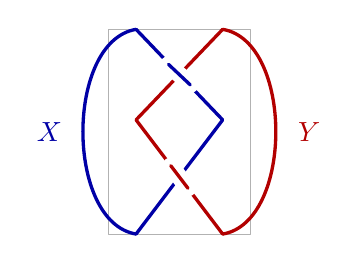
\begin{tikzpicture}[
    x=1cm,y=1cm,
    line cap=round,line join=round,
    strandX/.style={very thick,blue!65!black},
    strandY/.style={very thick,red!70!black}
]
    % Support of the local replacement.
    \draw[gray!60] (-0.9,-1.3) rectangle (0.9,1.3);

    % Componentwise exterior closure, shown explicitly.
    \draw[strandX]
        (-0.55,1.3)
        .. controls (-1.45,1.15) and (-1.45,-1.15) ..
        (-0.55,-1.3);
    \draw[strandY]
        (0.55,1.3)
        .. controls (1.45,1.15) and (1.45,-1.15) ..
        (0.55,-1.3);

    % The two strands of the full twist.
    \draw[strandX]
        (-0.55,1.3) -- (0.55,0.15) -- (-0.55,-1.3);
    \draw[strandY]
        (0.55,1.3) -- (-0.55,0.15) -- (0.55,-1.3);

    % X passes over at the upper crossing.
    \draw[white,line width=6pt] (-0.138,0.855) -- (0.138,0.595);
    \draw[strandX]               (-0.138,0.855) -- (0.138,0.595);

    % Y passes over at the lower crossing.
    \draw[white,line width=6pt] (-0.109,-0.432) -- (0.109,-0.718);
    \draw[strandY]              (-0.109,-0.432) -- (0.109,-0.718);

    \node[blue!65!black] at (-1.65,0) {\(X\)};
    \node[red!70!black] at (1.65,0) {\(Y\)};
\end{tikzpicture}
\caption{The componentwise closure of this tangle is a Hopf link.}
\label{fig:hopf-clasp}
\end{figure}

\begin{proof}
We first prescribe an abstract absolute linking matrix and then realize it by a
polygonal link.  Use frame components
\[
    R,F_1,\ldots,F_m,U,V
\]
and payload components
\[
    P_1,\ldots,P_m.
\]
The odd part of the absolute linking matrix is fixed as follows:
\[
    |\operatorname{lk}(R,U)|
    =
    |\operatorname{lk}(R,V)|
    =
    |\operatorname{lk}(R,F_1)|
    =
    1,
\]
\[
    |\operatorname{lk}(F_i,F_{i+1})|=1\quad(1\le i<m),
    \qquad
    |\operatorname{lk}(F_i,P_i)|=1\quad(1\le i\le m),
\]
and all other entries involving a frame component have even value \(0\).  Among
payload components set
\[
    |\operatorname{lk}(P_i,P_j)|=2a_{ij}.
\]

Reducing the absolute linking matrix modulo \(2\) gives a graph.  Its vertices
are the components; its edges are precisely the odd linking pairs above.  This
graph has only one nontrivial automorphism, namely the transposition of the two
leaves \(U,V\).  In particular it fixes \(R\), then fixes the path
\[
    F_1,F_2,\ldots,F_m
\]
in order, and therefore fixes each payload component \(P_i\).  Hence an
unoriented unordered ambient isotopy between two such links must identify the
payload submatrix entry-by-entry.  Since the payload entries are \(2a_{ij}\),
the matrix \(A\) is recovered from the ordinary unmarked link type.

It remains to realize the prescribed matrix with the stated stick cost.  Here
is a concrete routing model.  Write \(r=2m+3\) for the total number of frame
and payload components.  Place \(r\) distinct points \(v_i\) on the unit
circle in a horizontal plane.  Give component \(i\) a vertical rail through
\(v_i\), a return rail through \(2v_i\), and radial connectors above and
below a long vertical cylinder.  Before inserting clasps, the resulting
four-stick rectangles bound pairwise disjoint radial rectangles, so they
form an unlink.  Allocate disjoint thin horizontal slabs, one slab
for each required unit of linking.  In a slab assigned to components \(X,Y\),
leave every other rail straight and replace short subsegments of the \(X\)-
and \(Y\)-rails by an affine image of a fixed polygonal realization of the two-strand full twist
\(\sigma_1^2\), or its mirror \(\sigma_1^{-2}\), as in
Figure~\ref{fig:hopf-clasp}.  Its endpoints are matched to the original rail
segments on the same respective sides of the slab.  The supporting ball can
be a thin rectangular prism about the chord joining the two selected
\(v_i\): strict convexity of the circle ensures that this chord contains no
other rail point, and all return rails lie outside the unit disk.  Choose the
prism thin enough to miss every other rail and every return rail.  An affine
change of the fixed tangle changes its dimensions but not its number of
segments.  Distinct slab interiors are disjoint, and the radial closing
connectors lie above and below all slabs.  This gives the required uniform
stick cost even when the selected pair is far apart in the cross-section.

After choosing auxiliary orientations, choose between the two mirror-image
full twists so that its two crossings have positive sign.  The crossing
formula
\[
    \operatorname{lk}(X,Y)
    =\frac12\sum_{p\in X\cap Y}\operatorname{sign}(p)
\]
shows that each inserted twist raises \(\operatorname{lk}(X,Y)\) by one.
Because its supporting ball meets no other component, it changes no other
pairwise linking number.  Each component uses a fixed number of sticks for its
rail and return arc, and each clasp replaces two straight subsegments by a
fixed bounded number of sticks.  Thus a diagram
with \(q\) clasps has at most \(c_0m+c_1q\) sticks for universal constants
\(c_0,c_1\).  Since the final invariant uses absolute values, the auxiliary
orientations are irrelevant.  The fixed odd address graph uses \(O(m)\)
clasps, while the payload matrix uses
\(2\sum_{i<j}a_{ij}\) clasps.  Enlarging one universal constant \(B_0\) gives
the claimed estimate.
\end{proof}

\begin{theorem}[Unmarked unordered link production]\label{thm:link-lower}
There is an absolute positive integer \(B\) such that, for all \(n\ge2\),
\[
    |\Lcal_{Bn}|
    \ge
    \binom{\binom n2+n}{n}
    \ge
    n^n\exp(-O(n)).
\]
Consequently, for some constants \(c,C>0\),
\[
    N^{cN}\le |\Lcal_N|\le N^{CN}
\]
for all sufficiently large \(N\).
\end{theorem}

\begin{proof}
Take \(m=n\) in Proposition~\ref{prop:addressed-linking}, and consider all
nonnegative symmetric payload matrices with
\[
    \sum_{i<j}a_{ij}\le n.
\]
There are \(M=\binom n2\) independent entries, so the number of such matrices is
the stars-and-bars number
\[
    \binom{M+n}{n}.
\]
Each produces a distinct unmarked unordered link type, and each has total stick
number at most \(B n\) for a universal \(B\).  Finally,
\[
    \binom{M+n}{n}
    =
    \prod_{k=1}^n \frac{M+k}{k}
    \ge
    \frac{M^n}{n!}
    =
    n^n\exp(-O(n)),
\]
because \(M=\binom n2\).  The upper bound in the final display is
Remark~\ref{rem:link-upper}; the lower bound follows by replacing \(n\) by
\(\lfloor N/B\rfloor\).
\end{proof}

Thus ordinary unmarked unordered links already have the \(N^{\Theta(N)}\)
growth scale, with a completely elementary invariant: the absolute pairwise
linking matrix, together with a parity address frame that is itself part of the
unmarked link.

\section{Formal verification}

The Lean~4/mathlib development at
\url{https://github.com/sashakolpakov/StickNumbers} gives a conditional
certificate of the principal knot-counting deductions.  On the actual polygon
configuration space it verifies the cubic/quartic wall construction, path and
component logic, and, for \(N\ge5\), the explicit finite estimate behind the
\(N^{3N+o(N)}\) upper bound.  It also verifies the permutation family,
Garside-word bookkeeping, knot-transfer maps, the finite lower bound, the
headline \(\Theta(N\log N)\) law, and the eventual inequality
\(cN\log N\le\log|\Kcal_N|\) for every \(c<2/3\).  Here the bounded-stick
subtype belongs to a supplied knot-type interface, not to a formalized quotient
by ambient isotopy.  Generic support and isotopy invariance, Barone--Basu,
Garside normal-form theory, Malyutin--Stupakov, Huh--Oh, and orientation
reversal remain typed external theorems.  The internal floor/log calculation
for the \(-\frac23N\log\log N+O(N)\) refinement is also proved in Lean,
as is the eventual upper inequality with every coefficient greater than
\(3\); no additional arithmetic hypothesis is needed.  The auxiliary link
construction is outside the formal target.  The
repository contains the declaration-level audit and build instructions.

\section{Fewnomial and determinant directions}

The crossing equations have two special features.  First, each wall is a
constant-support polynomial: the affine four-point determinant
\(\det(p_b-p_a,p_d-p_c,p_c-p_a)\) has at most \(24\) monomial terms.  Second,
the family of all such walls is highly correlated: these are determinant walls
coming from one point configuration, not unrelated sparse cubics.  This places
the problem between fewnomial real algebraic geometry and the combinatorics of
order types.

One possible route is determinant-combinatorial.  The signs of all affine
four-point determinants are the chirotope data of the labeled configuration in
\(\R^3\).  Classical work of Goodman--Pollack gives
\(\exp(O(N\log N))\)-type bounds for fixed-dimensional point configurations
\cite{GoodmanPollack}.  Alon's refinement gives the fixed-dimensional
asymptotic order for configurations: for fixed \(d\), the number of labeled
order types of \(N\) points in \(\R^d\) has the form
\[
    N^{d^2N+o(N)}
\]
\cite{AlonMatroids}.  The same work gives \(N^{\Theta(N)}\) upper and lower
bounds for fixed-rank real matroids.  Thus affine order types in \(\R^3\) live
at scale \(N^{9N+o(N)}\), while rank-four vector matroid data live at
\(N^{\Theta(N)}\).  Our crossing discriminant uses only a structured subset of
the four-point determinant data.  This is why its count is much smaller than
the count of all order types.

There is an important distinction between counting determinant sign data and
counting chambers.  Order-type and oriented-matroid bounds count possible sign
patterns of minors.  The chamber count asks for connected components of
realization sets for such sign patterns, after intersecting with the stick-knot
discriminant complement.  Realization spaces of oriented matroids can be
topologically complicated by universality phenomena \cite{Mnev,RichterGebert};
hence matroid enumeration alone does not automatically give the chamber count.
The strong-geometry reconstruction theorem \cite{GrosRamirez} supplies a
different connection between enriched sign data and knot type.  Its
reconstruction statement is related geometric work; the component-counting
proof here works directly with the self-intersection walls and does not use
that theorem or assume that a wall sign vector classifies the knot.

A second route is genuinely fewnomial.  Existing fewnomial theorems control
positive solutions of sparse systems and the topology of sparse hypersurfaces
\cite{KhovanskiiFewnomials,BihanSottileFewnomial,BihanRojasSottile,
BihanSottileBetti}.  The chamber problem here asks for connected components of
sign conditions for \(O(N^2)\) sparse determinant walls on the Stiefel manifold.
The useful theorem would keep the dependence on the common sparse support and
the determinant incidence structure, rather than replacing the equations by an
arbitrary family of bounded-degree polynomials.

\begin{question}[Sparse determinant arrangement problem]
Can one prove a sign-condition component bound for the sparse determinant-wall
arrangement on \(\St_3(H)\) that improves the exponent or leading constant in
the \(N^{O(N)}\) bound of Theorem~\ref{thm:upper}?
\end{question}

There is also a lower-bound version of the same problem.  Fixing a regular
planar shadow, the over/under data are signs of height differences at its
crossings, hence are constrained by a finite system of linear inequalities in
the vertex heights.  This gives a concrete feasibility problem for crossing
assignments.  If one can construct shadows for which many feasible assignments
have distinct knot invariants, then the fewnomial/determinant chamber structure
would also become a knot production mechanism, not only an upper-bound
mechanism.

\section*{Acknowledgments}

The authors used OpenAI's GPT-5.6-sol as a research and coding assistant to
help strengthen the results, improve the exposition, and generate and audit
the Python and Lean~4 code accompanying this paper.  The authors reviewed the
resulting mathematics and code and take responsibility for the final content.

\begin{thebibliography}{99}

\bibitem{AdamsStick}
C. Adams, B. M. Brennan, D. L. Greilsheimer, and A. K. Woo,
``Stick numbers and composition of knots and links,''
\emph{Journal of Knot Theory and Its Ramifications} 6 (1997), 149--161.
\url{https://doi.org/10.1142/S0218216597000121}.

\bibitem{BochnakCosteRoy}
J. Bochnak, M. Coste, and M.-F. Roy,
\emph{Real Algebraic Geometry},
Ergebnisse der Mathematik und ihrer Grenzgebiete, vol. 36,
Springer, 1998.

\bibitem{AlonMatroids}
N. Alon,
``The number of polytopes, configurations and real matroids,''
\emph{Mathematika} 33 (1986), 62--71.
\url{https://web.math.princeton.edu/~nalon/PDFS/Publications2/The%20number%20of%20polytopes%2C%20configurations%2C%20and%20real%20matroids.pdf}.

\bibitem{BaroneBasu}
S. Barone and S. Basu,
``Refined bounds on the number of connected components of sign conditions on a variety,''
\emph{Discrete \& Computational Geometry} 47 (2012), 577--597.
\url{https://arxiv.org/abs/1104.0636}.

\bibitem{BihanRojasSottile}
F. Bihan, J. M. Rojas, and F. Sottile,
``On the sharpness of fewnomial bounds and the number of components of a fewnomial hypersurface,''
\url{https://arxiv.org/abs/math/0701667}.

\bibitem{BihanSottileFewnomial}
F. Bihan and F. Sottile,
``New fewnomial upper bounds from Gale dual polynomial systems,''
\emph{Moscow Mathematical Journal} 7 (2007), 387--407.
\url{https://arxiv.org/abs/math/0609544}.

\bibitem{BihanSottileBetti}
F. Bihan and F. Sottile,
``Betti number bounds for fewnomial hypersurfaces via stratified Morse theory,''
\emph{Proceedings of the American Mathematical Society} 137 (2009), 2825--2833.
\url{https://arxiv.org/abs/0801.2554}.

\bibitem{Calvo}
J. A. Calvo,
``Geometric knot spaces and polygonal isotopy,''
\emph{Journal of Knot Theory and Its Ramifications} 10 (2001), 245--267.
\url{https://arxiv.org/abs/math/9904037}.

\bibitem{CantarellaEtAl2025}
J. Cantarella, A. Rechnitzer, H. Schumacher, and C. Shonkwiler,
New upper bounds for stick numbers,
preprint, arXiv:2508.18263, 2025.
\url{https://arxiv.org/abs/2508.18263}.

\bibitem{EdwardsKirby}
R. D. Edwards and R. C. Kirby,
``Deformations of spaces of imbeddings,''
\emph{Annals of Mathematics} 93 (1971), 63--88.

\bibitem{ElrifaiMorton}
E. A. Elrifai and H. R. Morton,
``Algorithms for positive braids,''
\emph{Quarterly Journal of Mathematics} 45 (1994), 479--497.
\url{https://doi.org/10.1093/qmath/45.4.479}.

\bibitem{ErnstSumners}
C. Ernst and D. W. Sumners,
``The growth of the number of prime knots,''
\emph{Mathematical Proceedings of the Cambridge Philosophical Society} 102
(1987), 303--315.
\url{https://doi.org/10.1017/S0305004100067323}.

\bibitem{FreedmanHeWang}
M. H. Freedman, Z.-X. He, and Z. Wang,
\emph{M\"obius energy of knots and unknots},
\emph{Annals of Mathematics} 139 (1994), 1--50.
\url{https://doi.org/10.2307/2946626}.

\bibitem{GoodmanPollack}
J. E. Goodman and R. Pollack,
``Upper bounds for configurations and polytopes in \(\R^d\),''
\emph{Discrete \& Computational Geometry} 1 (1986), 219--228.
\url{https://eudml.org/doc/186385}.

\bibitem{GrosRamirez}
B. Gros and J. L. Ramirez Alfonsin,
\emph{Strong geometry: knots},
preprint, arXiv:2504.00197, version 3, 2025.
\url{https://arxiv.org/abs/2504.00197}.

\bibitem{HuhOh}
Y. Huh and S. Oh,
``An upper bound on stick numbers of knots,''
\emph{Journal of Knot Theory and Its Ramifications} 20 (2011), 741--747.
\url{https://doi.org/10.1142/S0218216511008966}.

\bibitem{KhovanskiiFewnomials}
A. G. Khovanskii,
\emph{Fewnomials},
Translations of Mathematical Monographs, vol. 88,
American Mathematical Society, Providence, RI, 1991.

\bibitem{KnotInfoStick}
KnotInfo,
``Stick number.''
\url{https://knotinfo.org/descriptions/polygon_index.html}.

\bibitem{MalyutinStupakovArc}
A. Malyutin and M. Stupakov,
``On the number of knots with a given arc index,''
PDMI preprint 07/2022.
\url{https://www.pdmi.ras.ru/preprint/2022/22-07.html}; full text:
\url{http://ftp.pdmi.ras.ru/pub/publicat/preprint/2022/07-22.pdf.gz}.

\bibitem{MillettPhysical}
K. C. Millett,
``Physical knot theory: an introduction to the study of the influence of
knotting on the spatial characteristics of polymers,''
selected lectures presented at the Abdus Salam International Centre for
Theoretical Physics, 2009; manuscript dated 2010.
\url{https://web.math.ucsb.edu/~millett/Preprints/MillettTriesteLectures.pdf}.

\bibitem{Mnev}
N. E. Mn\"ev,
``The universality theorems on the classification problem of configuration
varieties and convex polytopes varieties,''
in \emph{Topology and Geometry: Rohlin Seminar},
Lecture Notes in Mathematics, vol. 1346, Springer, 1988, 527--543.

\bibitem{RandellSimonTokle}
R. Randell, J. Simon, and J. Tokle,
M\"obius transformations of polygons and partitions of \(3\)-space,
\emph{Journal of Knot Theory and Its Ramifications} 17 (2008), 1401--1413.
\url{https://doi.org/10.1142/S0218216508006671}.

\bibitem{PollackRoy}
R. Pollack and M.-F. Roy,
``On the number of cells defined by a set of polynomials,''
\emph{Comptes Rendus de l'Acad\'emie des Sciences, S\'erie I} 316 (1993),
573--577.
\url{https://mariefrancoiseroy.pages.math.cnrs.fr/MFRoymathpublications.html}.

\bibitem{RichterGebert}
J. Richter-Gebert,
\emph{Realization Spaces of Polytopes},
Lecture Notes in Mathematics, vol. 1643, Springer, 1996.
\url{https://link.springer.com/book/10.1007/BFb0093761}.

\end{thebibliography}

\end{document}
